\documentclass[14pt]{extarticle}
\usepackage{fontspec}
\usepackage{polyglossia}
\usepackage{amsmath}
\usepackage{amssymb}
\usepackage{xcolor}
\usepackage{fancyhdr}
\usepackage{graphicx}
\usepackage{listings}
\usepackage[most]{tcolorbox}
% \usepackage{setspace}
\usepackage{pifont}
\usepackage{enumitem}
\usepackage{titlesec}
\usepackage[bottom]{footmisc}
\usepackage{titling}
\usepackage{minted}
\usepackage{etoolbox}
\usepackage{array}
\usepackage{extsizes}
\usepackage{float}
\usepackage{booktabs}
\usepackage{hyperref}
\usepackage[onehalfspacing]{setspace}
\usepackage[a4paper, top=2.7cm, bottom=2.7cm, left=2.5cm, right=2.5cm, headheight=1.5cm, headsep=0.5cm]{geometry}
\usepackage{tikz}

\usetikzlibrary{automata, positioning, arrows.meta, arrows}

\newfontfamily\emoji{Segoe UI Emoji}

\pagestyle{fancy}

\setmainlanguage[numerals=western]{arabic}
\setotherlanguage{english}
% \newfontfamily\arabicfont[Script=Arabic]{Amiri}
\newfontfamily\arabicfont[Script=Arabic]{Calibri}
\newfontfamily\arabicfonttt[Script=Arabic]{Courier New}

\lstset{
  language=[Sharp]C,
  numbers=left,
  stepnumber=1,
  numbersep=8pt,
  frame=single,
  basicstyle=\ttfamily\small,
  keywordstyle=\color{blue},
  stringstyle=\color{red},
  commentstyle=\color{green!50!black}
}

\newif\ifdetailed
\ifdefined\setdetailed
  \setdetailed
\fi

\newif\ifwithsols
\ifdefined\setwithsols
  \setwithsols
\fi

% unified tcolorboxes for articles
\tcbset{colback=white, colframe=black, fonttitle=\bfseries, boxrule=0.8pt}
\newtcolorbox{boxDef}[1][]{colback=blue!5!white,colframe=blue!75!black,
  title={{\emoji📘} تعريف\ifx\\#1\\\else ~#1\fi :}}
\newtcolorbox{boxExercise}[1][]{colback=cyan!5!white,colframe=cyan!70!black,
  title={{\emoji🧩} تمرين\ifx\\#1\\\else ~#1\fi :}}
\newtcolorbox{boxExample}[1][]{colback=yellow!5!white,colframe=orange!90!black,
  title={{\emoji📝} مثال\ifx\\#1\\\else ~#1\fi :}}
\newtcolorbox{boxNote}[1][]{colback=gray!10!white,colframe=black,
  title={{\emoji✨} ملاحظة\ifx\\#1\\\else ~#1\fi :}}
\newtcolorbox{boxAttention}[1][]{colback=magenta!10!white,colframe=magenta!80!black,
  title={{\emoji🔔} تنبيه\ifx\\#1\\\else ~#1\fi :}}
\newtcolorbox{boxWarning}[1][]{colback=red!5!white,colframe=red!75!black,
  title={{\emoji⚡} ملاحظة هامة\ifx\\#1\\\else ~#1\fi :}}
\newtcolorbox{boxSolution}[1][]{colback=green!5!white,colframe=green!60!black,
  title={{\emoji✅} حل\ifx\\#1\\\else ~#1\fi :}}
\newtcolorbox{boxSymbol}[1][]{colback=purple!5!white,colframe=purple!70!black,
  title={{\emoji🔣} رمز\ifx\\#1\\\else ~#1\fi :}}
\newtcolorbox{boxHint}[1][]{colback=teal!5!white,colframe=teal!60!black,
  title={{\emoji💡} تلميح\ifx\\#1\\\else ~#1\fi :}}


\tcbset{simplecode/.style={ colback=gray!5, colframe=black!50, boxrule=0.4pt, arc=2pt, left=4pt,right=4pt,top=4pt,bottom=4pt}}
\newenvironment{boxCode}{\begin{tcolorbox}[simplecode]}{\end{tcolorbox}}

\newcolumntype{C}[1]{>{\centering\arraybackslash}p{#1}}

% redefine spaces after titles
\makeatletter
\renewcommand{\@maketitle}{%
  \begin{center}
    {\huge \bfseries \@title \par}%
    \vskip 0.2em % space between title and author
    {\large \@author \par}%
    % \vskip 0.2em % space between author and date
    % {\normalsize \@date \par}%
  \end{center}
}
\makeatother

\fancyhf{} % clear default
\fancypagestyle{plain}{
  \fancyhf{}
  \fancyhead[L]{مدرسة التسامح الشاملة}
  % \fancyhead[L]{
\includegraphics[height=1cm]{../../../images/logoTasamoh.png}}
  \fancyhead[R]{الأستاذ محمود اغبارية}
  \fancyfoot[C]{\thepage}
}

\fancyhead[L]{مدرسة التسامح الشاملة}
\fancyhead[R]{الأستاذ محمود اغبارية}
\fancyfoot[C]{\thepage}
% \date{\today}

\setcounter{tocdepth}{3} % only section subsection and subsubsection in TOC

\newcommand{\importpdfpage}[2]{%
    \thispagestyle{empty}
    \newgeometry{left=0cm,right=0cm,top=0cm,bottom=0cm}
    \includegraphics[page=#2,width=0.95\paperwidth,height=0.95\paperheight,keepaspectratio]{#1}
    \restoregeometry
}

\newcommand{\insertFullImg}[1]{%
    \noindent
    \makebox[\textwidth][c]{
        \includegraphics[width=0.9\paperwidth,keepaspectratio]{#1}%
    }%
}%

% ----------------------


% \begin{document}

% \maketitle

% % \clearpage  % start TOC on a new page
% % \renewcommand{\contentsname}{جدول المحتويات}
% % \tableofcontents
% % \clearpage

% \part*{part 1} % the * prevents numbering
% \section*{مقدمة}
% \subsection*{مثال رياضي}
% \subsubsection*{مثال فرعي}
% \paragraph*{ paragraph 1}
% \subparagraph*{sub paragraph 1}

% \ifdetailed
% \begin{english}
% \begin{minted}{csharp}
% // C# Example
% \end{minted}
% \end{english}
% \fi

% OLD WAY
% \ifdetailed
% \begin{english}
% \begin{lstlisting}
% // C# Example
% \end{lstlisting}
% \end{english}
% \fi

% % 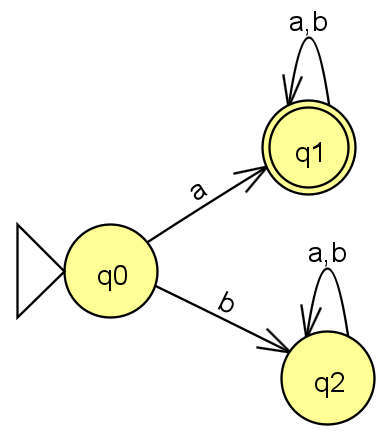
\includegraphics[width=0.2\textwidth]{../../../images/DFAs/ex1_q1.png}



% \vspace{3cm}
% \begin{flushleft}
% أرجو لكم وقتًا ممتعًا.

% الأستاذ محمود اغبارية.
% \end{flushleft}


% \end{document}


\title{ورقة مراجعة بايتون (أ)}
\date{}

\begin{document}

\maketitle
\thispagestyle{fancy}

\begin{enumerate}[itemsep=2em]
    \item
    معطى مقطع الكود التالي:
    \begin{boxCode}
    \begin{english}
    \begin{minted}{python}
num1 = int(input("Enter first number: "))
num2 = int(input("Enter second number: "))

print("Sum:", num1 + num2)
print("Floor Division:", num1 // num2)
print("Modulo:", num1 % num2)
    \end{minted}
    \end{english}
    \end{boxCode}
    ما هي المخرجات (الطباعة) التي ستظهر على الشاشة إذا أدخل المستخدم الأرقام 17 و 5 بالترتيب؟

    \item
    معطى مقطع الكود التالي:
    \begin{boxCode}
    \begin{english}
    \begin{minted}{python}
grade = int(input("Enter your grade: "))

if grade >= 90:
    print("Excellent")
elif grade >= 70:
    print("Good")
else:
    print("Needs improvement")
    \end{minted}
    \end{english}
    \end{boxCode}
    ماذا سيطبع البرنامج في كل من الحالات التالية:
    \begin{enumerate}[label=(\alph*)]
        \item إذا أدخل المستخدم 95.
        \item إذا أدخل المستخدم 75.
        \item إذا أدخل المستخدم 65.
    \end{enumerate}

    \item
    تتبع الكود التالي واكتب ماذا سيطبع إذا أدخل المستخدم الرقم 15:
    \begin{boxCode}
    \begin{english}
    \begin{minted}{python}
num = int(input("Enter a number: "))
if num > 10 and num % 2 == 0:
    print("Condition A")
elif num > 10 and num % 2 != 0:
    print("Condition B")
else:
    print("Condition C")
    \end{minted}
    \end{english}
    \end{boxCode}

    \item
    معطى مقطع الكود التالي:
    \begin{boxCode}
    \begin{english}
    \begin{minted}{python}
for i in range(1, 11):
    if i % 2 == 0:
        print(i, "is even")
    else:
        print(i, "is odd")
    \end{minted}
    \end{english}
    \end{boxCode}
    اكتب المخرجات (الطباعة) التي ستظهر على الشاشة عند تشغيل الكود، واشرح باختصار ماذا يفعل هذا البرنامج.

    \clearpage
    \item
    معطى مقطع الكود التالي:
    \begin{boxCode}
    \begin{english}
    \begin{minted}{python}
num = 345
hundreds = num // 100
tens = (num // 10) % 10
ones = num % 10

print("H:", hundreds)
print("T:", tens)
print("O:", ones)
    \end{minted}
    \end{english}
    \end{boxCode}
    ما هي المخرجات التي ستظهر على الشاشة؟ اشرح باختصار كيف تم استخراج منازل العدد باستخدام \texttt{//} و \texttt{\%}.

    \item
    تتبع الكود التالي واكتب ما هي المخرجات التي ستظهر على الشاشة. ما هو دور المتغير \texttt{sum}؟
    \begin{boxCode}
    \begin{english}
    \begin{minted}{python}
sum = 0
for i in range(1, 5):
    sum = sum + i
print("The result is:", sum)
    \end{minted}
    \end{english}
    \end{boxCode}

    \item
    معطى المتغير التالي:
    \begin{boxCode}
    \begin{english}
    \begin{minted}{python}
text = "Python is Fun"
    \end{minted}
    \end{english}
    \end{boxCode}
    ما هو ناتج تنفيذ الأوامر التالية؟
    \begin{enumerate}[label=(\alph*)]
        \item \texttt{print(len(text))}
        \item \texttt{print(text[0:6])}
        \item \texttt{print(text.upper())}
        \item \texttt{print(text.find("i"))}
    \end{enumerate}

    \clearpage
    \item
    معطى مقطع الكود التالي:
    \begin{boxCode}
    \begin{english}
    \begin{minted}{python}
num = 78643934
while num > 0:
    pair = num % 100
    print(pair)
    num = num // 100
    \end{minted}
    \end{english}
    \end{boxCode}
    تتبع الكود أعلاه واكتب المخرجات التي ستظهر على الشاشة. اشرح باختصار الفكرة من استخدام حلقة \texttt{while} مع \texttt{\%\ 100} و \texttt{//\ 100}.

    \item
    معطى مقطع الكود التالي:
    \begin{boxCode}
    \begin{english}
    \begin{minted}{python}
import random

count_six = 0
for i in range(10):
    dice = random.randint(1, 6)
    if dice == 6:
        count_six = count_six + 1

print("Number of 6s:", count_six)
    \end{minted}
    \end{english}
    \end{boxCode}
    إذا افترضنا أن الأرقام العشوائية التي تم سحبها بالترتيب هي (من اليسار إلى اليمين): \\
    $3, 6, 1, 6, 4, 6, 2, 5, 6, 1$ \\
    ماذا ستكون المخرجات (الطباعة) التي ستظهر على الشاشة في هذه الحالة؟ وما هو دور المتغير \texttt{count\_six}؟
\end{enumerate}


\end{document}
